\documentclass[diplomskirad]{fer}
% Dodaj opciju upload za generiranje konačne verzije koja se učitava na FERWeb
% Add the option upload to generate the final version which is uploaded to FERWeb
\usepackage{subcaption}

%--- PODACI O RADU / THESIS INFORMATION ----------------------------------------

\newtheorem{definicija}{Definicija}
\newtheorem{theorem}{Teorem}[chapter]
\newtheorem{algoritam}{Algoritam}
% Naslov na engleskom jeziku / Title in English
\title{Semidefinite programming relaxation for graph coloring and maximum clique number}

% Naslov na hrvatskom jeziku / Title in Croatian
\naslov{Relaksacije semidefinitnog programiranja za probleme bojanja grafova i maksimalne klike}

% Broj rada / Thesis number
\brojrada{819}

% Autor / Author
\author{Lana Šprajc}

% Mentor 
\mentor{prof. dr. sc. Josipa Pina Milišić}

% Datum rada na engleskom jeziku / Date in English
\date{June, 2025}

% Datum rada na hrvatskom jeziku / Date in Croatian
\datum{lipanj, 2025.}


%-------------------------------------------------------------------------------


\begin{document}


% Naslovnica se automatski generira / Titlepage is automatically generated
\maketitle


%--- ZADATAK / THESIS ASSIGNMENT -----------------------------------------------

% Zadatak se ubacuje iz vanjske datoteke / Thesis assignment is included from external file
% Upiši ime PDF datoteke preuzete s FERWeb-a / Enter the filename of the PDF downloaded from FERWeb
\zadatak{hr_0036532785_94.pdf}


%--- ZAHVALE / ACKNOWLEDGMENT --------------------------------------------------

\begin{zahvale}
  % Ovdje upišite zahvale / Write in the acknowledgment
  Hvala Branimiru na podsjetnicima da trebam pisati diplomski...
\end{zahvale}


% Odovud započinje numeriranje stranica / Page numbering starts from here
\mainmatter


% Sadržaj se automatski generira / Table of contents is automatically generated
\tableofcontents


%--- UVOD / INTRODUCTION -------------------------------------------------------
\chapter{Uvod}
\label{pog:uvod}

U teoriji grafova, problemi bojanja grafa i traženja maksimalne klike poznati su NP-teški problemi s brojnim primjenama. Bojanje grafa svakom vrhu 
grafa pridružuje jednu boju na način da su svaka dva susjedna vrha različitih boja. Svaki planar graf je moguće obojati u četiri boje \cite{fritsch1998four}.
Poznate primjene ovog problema su alociranje registara \cite{inproceedings}, raspoređivanje zadataka \cite{10.1093/comjnl/12.4.317}\dots

Problem traženja maksimalne klike je problem pronalaska potpuno povezanog podgrafa. Problem ima česte primjene u kemiji i bioinformatici,
primjerice za pronalaženje sličnih struktura u molekulama \cite{NAP4886}.

Za oba ova problema često je dovoljno pronaći rješenje koje je blizu optimalnom. Semidefinitno programiranja daje dobre aproksimacije rješenja problema
koje se mogu izračunati u polinomnoj složenosti.

Rad je podijeljen u 10 poglavlja. U drugom poglavlju dan je opširniji opis problema bojanja grafova
i traženja maksimalne klike kao i opis jednostavnih metoda rješavanja ovih problema.
U trećem poglavlju dan je pregled semidefinitnog programiranja i metoda rješavanja takvih problema.
U četvrtom poglavlju opisana je važnost Lovászovog broja i SDP formulacija za pronalazak njegove vrijednosti.
U petom poglavlju opisan je algoritam za bojanje grafova uz pomoć semidefinitnog programiranja.
U šestom poglavlju opisano je rješavanje problema pronalaska maksimalne klike uz primjenu semidefinitnog programiranja.
U sedmom poglavlju dan je pregled programskih ostvaranja i opis rada programa kroz primjere.
U osmom poglavlju prikazani su rezultati rada i mogućnosti daljnjeg rada u ovom području.
U devetom poglavlju dane su upute za prevođenje i pokretanje programa.
U desetom poglavlju iznesen je zaključak.

%-------------------------------------------------------------------------------
\chapter{Opis problema}
\label{opis_problema}

Graf se sastoji od $n$ vrhova i $m$ bridova. Pišemo $G = (V, E)$. Stupanj vrha je definiran kao broj vrhova s kojima je taj vrh susjedan. $\delta$ je
oznaka za najveći stupanj vrha.

\section{Bojanje grafova}
Bojanje grafa je postupak pridruživanja boje svakom vrhu grafa tako da su susjedni vrhovi različitih boja. Graf je $k$-obojiv ako postoji
bojanje grafa s $k$ ili manje boja. Kromatski broj $\chi(G)$ grafa je najmanji broj boja potreban za obojati graf. U većini primjena,
dovoljno je obojati graf s dovoljno malim brojem boja $k > \chi(G)$.

\subsection{$\delta + 1$ bojanje grafa}
\label{delta1}
$\delta + 1$ je jednostavan algoritan bojanja grafa koji boja graf s najviše $\delta + 1$ bojom. Algoritam je složenosti $O(n^2)$.
Neka je $\{1, \dots, \delta + 1\}$ skup boja. Svakom vrhu pridružuje se najmanji broj kojim nije obojan ni jedan od njegovih susjeda. Uvijek će postojati
barem jedna takva boja jer svaki vrh ima najviše $\delta$ susjeda, a postoji $\delta + 1$ boja. Problem ovog algoritma je što je u većini slučajeva 
kromatski broj grafa puno manji od $\delta + 1$.

\section{Traženje maksimalne klike}
Klika u grafu je potpuno povezani podgraf. Maksimalna klika (engl. \textit{maximum clique}) je najveći takav podgraf. Broj vrhova u maksimalnoj kliki označavamo s $\omega(G)$.
Ovaj broj predstavlja donju granicu kromatskog broja grafa, $\omega(G) \leq \chi(G)$.

Lokalno maksimalna klika (engl. \textit{maximal clique, inclusion-maximal}) je klika koja nije podgraf veće klike. Takvoj kliki nije moguće dodati ni jedan
vrh grafa koji nije dio klike, na način da dobiveni podgraf ostaje klika.

\subsection{Pohlepno traženje lokalno maksimalne klike}
\label{pog:greedy_clique}
Jednostavan algoritam za traženje lokalno maksimalne klike započinje proizvoljno odabranim vrhom, tj. skupom $S = \{v\}$.
Algoritam zatim iterira kroz preostale vrhove grafa i za svaki vrh $w$ provjerava čini li podgraf $S \cup \{ w \}$ kliku. 
Ako čini, vrh $w$ dodaje se u skup $S$; u suprotnom se odbacuje.

\chapter{Semidefinitno programiranje}
\label{pog:semidefinitno_programiranje}
Semidefinitno programiranje (krat. \textit{SDP}) klasa je optimizacijskih problema.
Standardni oblik problema je:

\begin{equation}
\begin{split}
  & min f = \langle CX \rangle \\
  t. d. & \langle A_iX \rangle = b_i \\
        & X = X^T \succeq 0
\end{split}
\end{equation}
pri čemu $ \langle A \rangle = \sum_{i}^{n} a_{i,i} $
označava trag kvadratne matrice. $X \succeq 0$ označava da je matrica pozitivno semidefinitna.

Dualni problem zadan je jednadžbama: 
\begin{equation}
\begin{split}
  & min \sum_{i}^{m} b_iy_i \\
  t.d. & \sum_{i}^{m} A_iy_i + Z = C \\
      & Z \succeq 0 \\
\end{split}
\end{equation}

Semidefinitno programiranje ima primjene u rješavanju problema makimalnog reza (engl. \textit{max cut problem}) \cite{7804990}, u rješavanju SAT problema \cite{doi:10.3233/SAT190001} \dots %TODO mozda jos neke primjene

\section{Teorija dualnosti}
U optimizacijskim problemima, razmak dualnosti (engl. \textit{duality gap}) je razlika između optimuma primarnog $p^*$ i dualnog $d^*$ problema, $p^* - d^*$.
Kažemo da vrijedi slaba dualnost ako je razmak dualnosti veći ili jednak od 0. Jaka dualnost vrijedi ako su optimum primarnog i dualnog problema jednaki, to jest
ako je razmak dualnosti jednak 0 \cite{HINTERMULLER2019437}.

Za SDP razmak dualnosti jednak je:
\begin{equation}
  \begin{split}
    \langle CX \rangle - b^Ty &= \langle(\sum_{i=1}^{m}A_iy_i + Z)X \rangle - b^Ty \\
    &= \langle ZX \rangle + \sum_{i=1}^{m}(\langle A_iX \rangle - b_i) y_i \\
    &= \langle ZX \rangle \geq 0
  \end{split}
\end{equation}

Iz ovoga je vidljivo da za SDP vrijedi slaba dualnost, ali ne nužno i jaka. Prema Slaterovom uvjetu, jaka dualnost je zadovoljena ako postoji rješenje primarnog problema u kojem je
zadovoljen uvjet $X \succ 0$ i rješenje dualnog problema takvo da vrijedi $Z \succ 0$ \cite{slater}.

\section{Metode rješavanja SDP}
Postoje razne metode rješavanja SDP-a, primjerice elipsoidna metoda i metoda unutarnje točke. Ove metode numerički pronalaze rješenje, obično u polinomnoj složenosti.

\subsection{Metoda unutarnje točke}
Kao što ime kaže, metoda unutarnje točke započinje točkom unutar prostora koji zadovoljava uvjete semidefinitnog programa i postupno se priližava optimumu.
Algoritam definira zamjensku funkciju za optimizaciju $f^*(x) = f(x) + b(x)$, gdje je $b(x)$ takozvana granična funkcija. $b(x)$ teži beskonačnosti kako se
$x$ približava granici dopuštenog prostora, dok unutar prostora problema ima malu vrijednost blizu 0. 
Optimizacijski algoritmi izbjegavaju rubni prostor problema i pronalaze optimum unutar dozvoljenog prostora.

\chapter{Lovászov broj}
\label{pog:lovaszov_broj}
Lovászov broj (Lovászova theta funkcija) rješenje je sljedećeg semidefinitnog programa:
\begin{equation}
  \begin{split}
    & \theta = \max \langle JX \rangle \\
    t.d. & \langle X \rangle = 1 \\
         & x_{i,j} = 0, \forall (i,j) \in E(G) \\
         & X=X^T \succeq 0 
  \end{split}
\end{equation}

Ovdje J predstavlja $n \times n$ matricu ispunjenu jedinicama.


Za Lovászov broj, $ \theta(G) $ vrijedi da je veći od ili jednak broju klike, a manji od ili jednak kromatskom broju grafa, 
$\omega(G) \leq \theta(G) \leq \chi(G)$. \cite{1055985}

Ovaj program se pretvora u standardnu formu tako da se postavi $C = -J$, $A_1 = I$, $b_1 = 1$,
$A_i = E_{j,k}, \forall (j,k) \in E(G)$, $b_i = 0, i \in \{2, \dots, m\}$. Ovdje $E_{i,k}$ predstavlja matricu koja sadrži 0 na
svim mjestima osim na $e_{i,j}$ i $e_{j, i}$ gdje sadrži 1.


\chapter{Primjene SDP-a u bojanju grafova}
\label{pog:primjene_SDP-a_u_bojanju_grafova}

U formulaciji bojanja grafova pomoću SDP-a, vrhovima se pridružuju jedinični vektoru. Vektori pridruženi susjednim vrhovima moraju
biti udaljeni jedan od drugog.

\begin{definicija} (iz \cite{karger1998approximategraphcoloringsemidefinite})
  Za graf G=(V, E) s n vrhova i m bridova i realni broj $k \geq 1$, vektorsko k-bojanje je pridruživanje jediničnih
  vektora $v_i \in \Re^n$ svakom vrhu $i$ grafa G takvih da za svaka dva susjedna vrha $v_{i,j} \in E$ vrijedi:
  \begin{equation}
    v_i \cdot v_j \leq - \frac{1}{k-1}
  \end{equation}
\end{definicija}

\begin{definicija} (iz \cite{karger1998approximategraphcoloringsemidefinite})
  Za graf G=(V, E) s n vrhova i m bridova i realni broj $k \geq 1$, matrično k-bojanje je određivanje simetrične pozitivno semidefinitne matrice M,
  takve da je $m_{i,i} = 1, i \in \{1, \dots, n\}$ i $m_{i,j} = m_{j,i} \leq - \frac{1}{k-1}, (i, j) \in E$.
\end{definicija}

Matrično k-bojanje i vektorsko k-bojanje su ekvivalentni. Ako je poznato vektorsko k-bojanje, matrica M određuje se tako da se
element $m_{i,j}$ postavi na skalarni produkt vektora $v_i$ i $v_j$. Ako je poznato matrično k-bojanje, matricu $M$ moguće je faktorizirati
pomoću dekompozicije svojstvenim vrijednosti (engl. \textit{eigendecomposition}) tako da vrijedi $M = VV^T$. Sada su stupci matrice $V$ jedinični
vektori koji čine vektorsko k-bojanje grafa. \cite{karger1998approximategraphcoloringsemidefinite}

\section{Važnost vektorskog bojanja grafa}
\begin{theorem}\label{teorem1}
  Za $k \leq n$, postoji k jediničnih vektora $v_i \in \Re^n$ takvih da je $v_i \cdot v_j = -\frac{1}{k-1}, \forall i \neq j$ 

  \textbf{Dokaz} (iz \cite{karger1998approximategraphcoloringsemidefinite}) Dovoljno je dokazati da ovo vrijedi za k = n, ako je k manji od n
  $v_{i}[j]$ se postavlja na 0 za sve j > k.

  Konstruirani su vektori $v_1, \dots, v_k$ na sljedeći način:

  \begin{equation}
    v_i[j] = \begin{cases} -\sqrt{\frac{1}{k(k-1)}} & j \neq i \\ \sqrt{\frac{k-1}{k}} & j = i \end{cases}
  \end{equation}
\end{theorem}

\begin{theorem}
  Svaki k-obojiv graf je i vektorski k-obojiv.

  \textbf{Dokaz} (iz \cite{karger1998approximategraphcoloringsemidefinite}) Graf je uvijek obojiv s $k \leq n$ boja jer je u najgorem slučaju
  svaki vrh obojan u različitu boju. Svakom vrhu obojanom s $i$-tom bojom, pridružuje se vektor $v_i$ iz \ref{teorem1}.
\end{theorem}

Iz ovog teorema vidljivo je da je minimalni k za koji je graf vektorski k-obojiv donja granica za kromatski broj grafa.

\section{Formulacija SDP}
Slijedi SDP formulacija vektorskog bojanja grafa koja minimizira k za koji je graf vektorski k-obojiv.

\begin{equation} \label{eq:color_notstandard}
  \begin{split}
    & \min \alpha \\
    t.d. & x_{ii} = 1 \\
         & x_{ij} \leq \alpha, \forall (i,j) \in E(G) \\
         & X=X^T \succeq 0 
  \end{split}
\end{equation}

Optimalni $\alpha$ jednak je $-\frac{1}{k-1}$. Kako bi problem bio u standardnoj formi, u matrici $X$ uvodi se novi element na dijagonalu tako da
$x_{n+1,n+1} = \alpha$. Dodatno, uvode se \textit{slack} varijable za uvjete povezane s bridovima. Konačna formulacija problema u standarnoj formi je: 


\begin{equation} \label{sdpbojanje}
  \begin{split}
    & \min \langle E_{n+1,n+1}X \rangle \\
    t.d. & \langle E_{ii}X \rangle = 1 \\
         & \langle E_{ij}X \rangle - 2 \langle E_{n+1,n+1}X \rangle + \langle E_{n+1+k,n+1+k}X \rangle = 0, \forall (i,j) \in E(G), k \in \{1,\dots,m\} \\
         & X=X^T \succeq 0 
  \end{split}
\end{equation}

\section{Pretvorba vektorskog bojanja u bojanje grafa}
Rješavanjem SDP-a dobiva se vektorsko bojanje grafa koje je potrebno pretvoriti u bojanje grafa. Postoji nekoliko algoritma za ovaj problem. Neki od njih su metoda odsijecanja ravninama 
(engl. \textit{cutting plane method}) i zaokruživanje vektorskim projekcijama.

\subsection{Semibojanja}
\begin{definicija}
  k-semibojanje (engl. \textit{k-semicoloring}) grafa G je pridruživanje k boja barem polovici vrhova grafa G tako da dva susjedna vrha nisu jednake boje. 
\end{definicija}

Ako je poznato k-semibojanje grafa, tada je moguće obojati cijeli graf u $k\log n$ boja. Ovo je moguće rekurzivnim bojanjem barem polovice preostalog grafa,
sve dok ne ostanu jedan ili nijedan neobojan vrh.

\subsection{Metoda odsijecanja ravninama}
Motivacija algoritma je činjenica da su vektori koji predstavljaju susjedne vrhove udaljeni u prostoru, to jest velik je kut između njih.
Generira se $N$ slučajnih hiperravnina koje prolaze kroz ishodište koordinatnog sustava. One dijele prostor na $2N$ dijelova. Svakom dijelu je pridružena
jedna boja te su svi vektori u tom prostoru obojani tom bojom. Ukoliko su dva susjedna vrha obojana istom bojom, jednom od tih vrhova treba maknuti boju.

Vjerojatnost da su 2 susjedna vrha s različitih strana jedne hiperravnine je $\beta / \Pi$, gdje je $\beta$ kut između vektorskih reprezentacija
tih vektora. Za veći broj hiperravnina, smanjuje se vjerojatnost da su vrhovi u jednakim podprostorima.
Budući da susjedni vektori imaju velike kuteve između vektorskih reprezentacija, oni imaju manju vjerojatnost da se nalaze u jednakim podprostorima.
Promijenom parametra $N$ bira se između točnog bojanja većeg broja vrhova za veći $N$ i bojanja s manjim brojem boja za manji $N$. \cite{karger1998approximategraphcoloringsemidefinite} 


\subsection{Zaokruživanje vektorskim projekcijama}
\label{pog_vektorske_projekcije}
U ovom algoritmu, traže se veliki podgrafi u kojima ni jedan vrh nije međusobno povezan. Zadovoljavajuće je pronaći podgraf s N vrhova i m bridova,
gdje je $N >> m$ te izbaciti m vrhova koji su imaju susjedne vrhove u podgrafu. Ovih $N - m$ vrhova možemo obojati jednom bojom.

\begin{algoritam} Bojanje grafa vektorskim projekcijama
  \begin{enumerate}
    \item generiranje slučajnog vektora \textbf{u} po standardnoj distribuciji i normaliziracija
    \item ako je $|v_i \cdot u| > \epsilon$, dodavanje vrha \textbf{i} u trenutni skup vrhova 
    \item provjera nalaze li se bridovi u dobivenom podgrafu i izbacivanje potrebnih vrhova iz skupa
    \item bojanje trenutnog skupa vrhova u jednu boju
    \item ponavljanje dok nisu obojani svi vrhovi
  \end{enumerate}
\end{algoritam}

Intuitivno, ako je jedan od vektora $v_i$ blizu slučajnom vektoru $u$, tada su njegovi susjedni vektori $v_j$ koji su udaljeni od vektora $v_i$, vjerojatno
udaljeni i od vektora $u$. Promijenom parametra $\epsilon$ utječemo na broj obojenih vektora u jednom koraku, ali i broj \textit{uhvaćenih} bridova.

\section{Wigdersonova tehnika}
Algoritmi bojanja grafova mogu se poboljšati korištenjem Wigdersonove tehnike.
Algoritam određuje konstantu $\beta$ i ako postoji vrh stupnja većeg od $\beta$, on i njegovi susjedi bojaju se s 2 boje koje se dalje više ne
koriste. \cite{2002_Wigderson} Ovo smanjuje maksimalni stupanj bojanog podgrafa, a broj boja koje algoritmi koriste ovisi o maksimalnom stupnju
grafa pa se primjenom ove tehnike smanjuje taj broj.

\chapter{Primjene SDP-a u traženju maksimalne klike}
\label{pog:primjene_SDP-a_u_traženju_maksimalne_klike}

Stabilan skup (engl. \textit{stable set}) je podskup vrhova grafa G koji ne sadrži dva susjedna vrha. Inverzni graf $\bar{G}$ grafu $G$ 
sastoji se od jednakog skupa vrhova kao i graf $G$. Vrhovi $v_i$ i $v_j$ u grafu $\bar{G}$ su povezani ako i samo ako nisu povezani u grafu $G$.

Skup vrhova S je klika u grafu $G$ ako i samo ako je stablian skup u grafu $\bar{G}$. Dakle, problem maksimalne klike grafa G ekvivalentan je
problemu maksimalnog stabilnog skupa grafa $\bar{G}$. \cite{article}

U nastavku je opisana metoda pronalska maksimalnog stabilnog skupa.

\section{SDP formulacija problema maksimalnog stabilnog skupa}
Svakom vrhu grafa pridjeljuje se vrijednost $-1$ ili $1$. Jedan od ovih skupova predstavlja stabilan skup. Grafu se dodaje jedan vrh $v_{n+1}$ koji
nije povezan ni s jednim vrhom grafa G. Ovaj vrh se očito nalazi u maksimalnom stabilnom skupu. Vrh služi prepoznavanju koji od skupova
je stabilan skup.

Problem je definiran na sljedeći način (iz \cite{article}):
\begin{equation}
  \begin{split}
    & \max \frac{1}{2} \sum_{i=1}^{n} (v_i^2+v_{n+1}v_{i}) \\
    t.d. & v \in \{-1, 1\}^{n+1} \\
         & |v_i+v_j+v_{n+1}| = 1 \forall (i, j) \in E
  \end{split}   
\end{equation}

Izraz $v_i^2+v_{n+1}v_{i}$ je jednak 0 ako je $v_i$ različitog predznaka kao i $v_{n+1}$ ili jednak 2 ako je $v_i$ jednakog predznaka kao i $v_{n+1}$.
Što znači da je vrijednost optimizacijske funkcije jednaka broju vrhova u maksimalnom stabilnom skupu.

Problem se relaksira u SDP na sljedeći način (iz \cite{article}):
\begin{equation} \label{eq1}
  \begin{split}
    & \max \Biggl \langle \begin{bmatrix}
      .5 & & & .25 \\
      & \ddots &  & \vdots \\
      & & .5 & .25 \\
      .25 & \cdots & .25 & 0
    \end{bmatrix} X \Biggr \rangle \\
    t.d. & diag(X) = e \\
    &  \langle (e_{ijk} e_{ijk}^T) X \rangle = 1 \\
    & X = X^T \succeq 0 
  \end{split}
\end{equation}

Iz relaksiranog problema dobiva se stabilni skup prateći sljedeći algoritam:
\begin{algoritam} Određivanje maksimalnog stabilnog skupa
  \label{maks_clique}
  \begin{enumerate}
    \item Iz optimalnog $X^*$ dobivenog iz \ref{eq1} određuje se V za koji vrijedi $X^* = VV^T$
    \item Za slučajan jedinični vektor $u \in \Re^{n+1}$ računa se $v = sign(Vu)$
    \item Za svaki $(i,j) \in E$, ako ne vrijedi $|v_i+v_j+v_{n+1}| = 1$, mijenja se prednjak od $v_i$ ili $v_j$, onom kojem je vrijednost $V_{k}u$ udaljenija od $V_{n+1}u$
  \end{enumerate}
\end{algoritam}

Stabilan skup vrhova je onaj skup vrhova koji imaju jednaki predznak kao i $v_{n+1}$.

\chapter{Programska ostvarenja}
\label{pog:programska_ostvarenja}

U sklopu rada implementiran je algoritam za bojanje grafova i traženje maksimalne klike.
Implementiran je program za vizualizaciju grafa i program za generiranje slučajnih grafova.

Sav kod napisan je u C++-u uz korištenje biblioteke DSDP \cite{dsdp-user-guide} i OpenBLAS implementacije BLAS/LAPACK paketa \cite{openBLAS}.

Definirana je klasa \verb|Graph| koja učitava graf spremljen u datoteci u obliku matrice susjedstva. U ovom zapisu,
jedinica predstavlja da postoji brid između dva vrha, dok nula predstavlja da vrhovi nisu povezani. Definirane su metode \verb|color| koja boja graf
algoritmom zaokruživanja vektorskim projekcijama, \verb|greedy_color| koja boja graf $\delta + 1$ algoritmom, \verb|find_max_clique| koja
pronalazi veliku kliku SDP relaksacijom i \verb|greedy_clique| koja pronalazi lokalno maksimalnu kliku.

Kod je moguće pronaći na \cite{key}.

\section{Bojanje grafova}
Implementirana su dva algoritma za bojanje grafova: SDP relaksacijom uz zaokruživanje vektorskim projekcijama i $\delta + 1$ algoritmom.

$\delta + 1$ algoritam je implementiran kao što je objašnjeno u poglavlju \ref{delta1}.

Za bojanje zaokruživanjem vektorskih projekcijama, u problemu \ref{eq:color_notstandard} uvjeti nejednakosti pretvoreni su u jednakosti kako bi se
ubrzao rad programa. Problem je pretvoren u standardnu formu na sljedeći način:
\begin{equation} \label{eq:color_relaxed}
  \begin{split}
    & \min \langle E_{n+1,n+1}X \rangle \\
    t.d. & \langle E_{ii}X \rangle = 1 \\
         & \langle E_{ij}X \rangle - 2 \langle E_{n+1,n+1}X \rangle = 0, \forall (i,j) \in E(G) \\
         & X=X^T \succeq 0 
  \end{split}
\end{equation}
Problem \ref{eq:color_relaxed} rješen je korištenjem biblioteke DSDP \cite{dsdp-user-guide}.
Korištenjem ove biblioteke dobivena je optimalna matrica $X$ koja je faktorizirana u oblik $VV^T$ korištenjem
OpenBLAS-a \cite{openBLAS}.

Graf je dalje obojan kako je opisano u poglavlju \ref{pog_vektorske_projekcije}. Nije korištena Wigdersonova tehnika.

\subsection{Primjer bojanja grafa}
Zaokruživanje vektorskim projekcijama objašnjeno je na grafu G s tablicom susjedstva \ref{matrica_susjeda}.
Na slici \ref{grafG} prikazan je graf G s oznakama vrhova
0, \dots, 9.

\begin{equation} \label{matrica_susjeda}
   G =\begin{pmatrix}
    1 & 0 & 0 & 0 & 0 & 0 & 1 & 1 & 0 & 1 \\
    0 & 0 & 1 & 1 & 0 & 0 & 0 & 0 & 1 & 0 \\
    0 & 1 & 0 & 0 & 1 & 0 & 1 & 1 & 1 & 0 \\
    0 & 1 & 0 & 1 & 0 & 0 & 0 & 0 & 0 & 0 \\
    0 & 0 & 1 & 0 & 0 & 0 & 0 & 0 & 0 & 1 \\
    0 & 0 & 0 & 0 & 0 & 0 & 0 & 1 & 1 & 1 \\
    1 & 0 & 1 & 0 & 0 & 0 & 0 & 0 & 0 & 1 \\
    1 & 0 & 1 & 0 & 0 & 1 & 0 & 0 & 1 & 1 \\
    0 & 1 & 1 & 0 & 0 & 1 & 0 & 1 & 0 & 1 \\
    1 & 0 & 0 & 0 & 1 & 1 & 1 & 1 & 1 & 1 \\
  \end{pmatrix}
\end{equation}

\begin{figure}
  \centering
  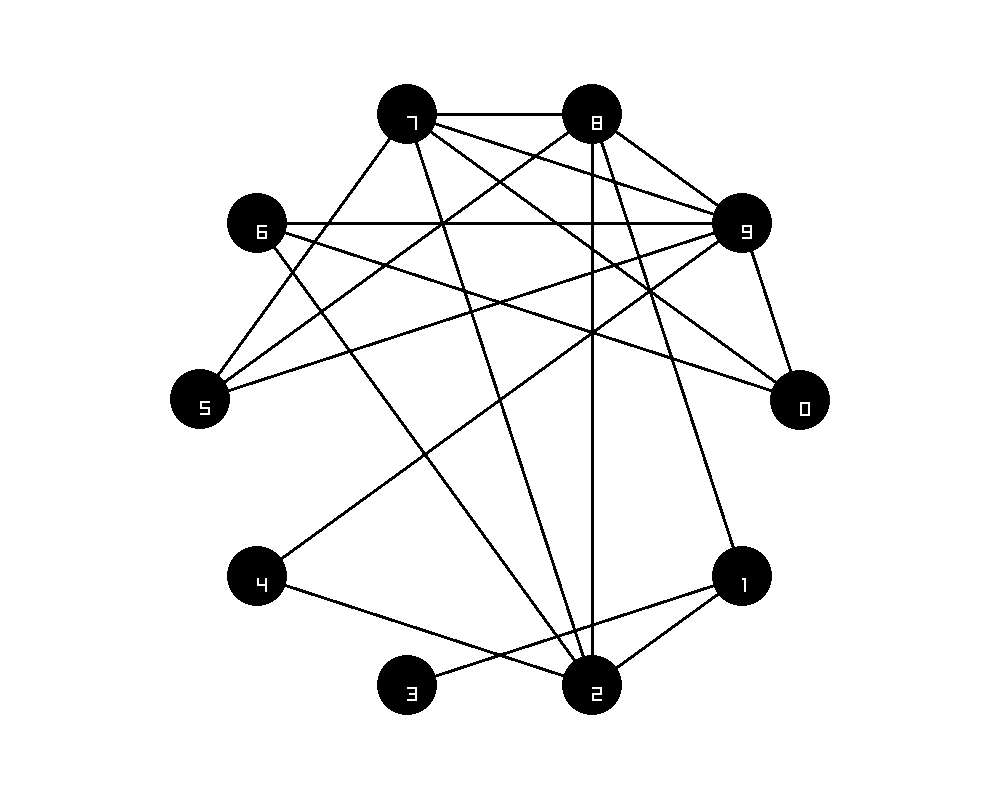
\includegraphics[scale=0.4]{images/colors_it2.png}
  \caption{Prikaz grafa G}
  \label{grafG}
\end{figure}

U tablici \ref{vekt_bojanje} prikazano je vektorsko bojanje grafa G koje se dobiva rješavanjem pripadajućeg SDP-a.
U tablici \ref{sluc_vekt} prikazani su slučajni vektori generirani u postupku bojanja grafa G zaokruživanjem vektorskim projekcijama.
U tablici \ref{skalar} prikazani su skalarni umnošci iterativno generiranih slučajnih vektora s vektorima pripadajućih vrhova grafa G.
Vrijednost parametra $\epsilon = 0.0$. U prvom koraku vrhovi 6, 7 i 8 imaju skalarni produkt $>\epsilon$. Budući da su vrhovi 7 i 8 susjedni, 
vrh 8 nije obojan. Na slici \ref{prvo_bojanje}, prikazan je graf nakon prve iteracije bojanja.

U drugom koraku, vrhovi 2, 3, 4, 8 i 9 imaju skalarni produkt $>\epsilon$. Vrhovi 4 i 8 nisu obojani jer postoje bridovi (2, 4), (4, 9) i (8, 9).
Slika \ref{drugo_bojanje}, prikazuje graf G nakon druge iteracije bojanja.

U trećoj iteraciji, vrhovi 0, 1, 4 i 8 imaju pozitivni skalarni produkt. Vrh 8 nije obojan zato što postoji brid (1, 8). Na slici \ref{trece_bojanje}
prikazan je graf G nakon trećeg koraka algoritma bojanja grafa.

Ostali su vrhovi 5 i 8 koji su povezani pa su oni obojani različitim bojama u sljedeće dvije iteracije algoritma. Na slici \ref{zadnje_bojanje}
prikazan je potpuno obojan graf G.

\begin{table}[h]
  \caption{Vektorsko bojanje grafa G}
  \label{vekt_bojanje}
  \centering
  \resizebox{\columnwidth}{!}{
  \begin{tabular}{|c|c|c|c|c|c|c|c|c|c|c|c|}
    \hline
    i & $v_{i,0}$ & $v_{i,1}$ & $v_{i,2}$ & $v_{i,3}$ & $v_{i,4}$ & $v_{i,5}$ & $v_{i,6}$ & $v_{i,7}$ & $v_{i,8}$ & $v_{i,9}$ \\
    \hline
    \hline
    0 & 0.000 & 0.226 & -0.253 & 0.113 & -0.340 & 0.0680 & 0.286 & 0.342 & 0.627 & 0.401 \\
    \hline
    1 & 0.000 & -0.191 & -0.174 & 0.475 & -0.024 & 0.026 & 0.387 & 0.410 & -0.364 & -0.506 \\
    \hline
    2 & 0.000 & -0.174 & -0.387 & -0.276 & 0.069 & -0.003 & -0.232 & 0.153 & -0.300 & 0.756 \\
    \hline
    3 & 0.000 & -0.021 & -0.043 & 0.518 & -0.041 & 0.273 & -0.657 & -0.327 & 0.218 & 0.259 \\
    \hline
    4 & 0.000 & 0.037 & -0.126 & -0.126 & 0.539 & 0.570 & 0.084 & 0.075 & 0.404 & -0.419 \\
    \hline
    5 & -0.010 & -0.042 & 0.207 & 0.070 & 0.204 & -0.116 & -0.198 & 0.806 & 0.278 & 0.358 \\
    \hline
    6 & 0.000 & 0.151 & -0.236 & 0.057 & 0.258 & -0.564 & -0.355 & 0.056 & 0.046 & -0.634 \\
    \hline
    7 & -0.010 & 0.017 & -0.076 & -0.223 & -0.425 & 0.270 & -0.301 & 0.107 & -0.244 & -0.728 \\
    \hline
    8 & -0.010 & -0.174 & -0.087 & -0.003 & 0.006 & -0.218 & 0.257 & -0.591 & 0.705 & -0.049 \\
    \hline
    9 & -0.010 & 0.192 & -0.048 & 0.158 & 0.216 & 0.062 & 0.245 & -0.320 & -0.741 & 0.416 \\
    \hline
  \end{tabular}
  }
\end{table}

\begin{table}[h]
 \caption{Generirani slučajni vektori $r_i$}
 \label{sluc_vekt}
  \begin{tabular}{|c|c|c|c|c|c|c|c|c|c|c|c|}
    \hline
    i & $r_{i,0}$ & $r_{i,1}$ & $r_{i,2}$ & $r_{i,3}$ & $r_{i,4}$ & $r_{i,5}$ & $r_{i,6}$ & $r_{i,7}$ & $r_{i,8}$ & $r_{i,9}$ \\
    \hline
    \hline
    0 & 0.057 & -0.219 & 0.846 & 0.061 & 0.000 & -0.252 & -0.052 & -0.254 & 0.039 & -0.312 \\
    \hline
    1 & -0.556 & -0.436 & 0.246 & -0.042 & 0.191 & 0.479 & 0.225 & -0.270 & 0.124 & 0.186 \\
    \hline
    2 & -0.260 & 0.172 & -0.272 & 0.320 & 0.250 & 0.643 & 0.159 & -0.395 & 0.261 & -0.039 \\
    \hline
    3 & 0.195 & -0.327 & 0.190 & -0.060 & -0.415 & -0.060 & -0.229 & 0.603 & 0.460 & -0.105 \\
    \hline
    4 & -0.011 & 0.019 & 0.732 & 0.432 & -0.015 & -0.312 & 0.146 & -0.000 & 0.289 & 0.274\\
    \hline
    \end{tabular}
\end{table}

\begin{table}[h]
  \caption{Umnošci slučajnih vektora s vektorima vrhova}
  \label{skalar}
  \begin{tabular}{|c|c|c|c|c|c|c|c|c|c|c|c|}
    \hline
    i & $r_i \cdot v_0 $ & $r_i \cdot v_1 $ & $r_i \cdot v_2 $ & $r_i \cdot v_3 $ & $r_i \cdot v_4 $ & $r_i \cdot v_5 $ & $r_i \cdot v_6 $ & $r_i \cdot v_7 $ & $r_i \cdot v_8 $ & $r_i \cdot v_9 $ \\
    \hline
    \hline
    0 & -0.476 & -0.063 & -0.580 & -0.024 & -0.143 & -0.078 & 0.117 & 0.056 & 0.199 & -0.179 \\
    \hline
    1 & -0.073 & -0.135 & 0.014 & 0.115 & 0.304 & -0.107&& & 0.252 & 0.102 \\
    \hline
    2 & 0.161 & 0.002 & & & 0.607 & -0.353 & & & 0.316 & \\
    \hline
    3 & & & & & & 0.591 & & & -0.037 & \\
    \hline
    4 & & & & & & & & & 0.228 & \\
    \hline
  \end{tabular}
\end{table}

\begin{figure}
  \centering
  \begin{subfigure}[b]{0.4\linewidth}
    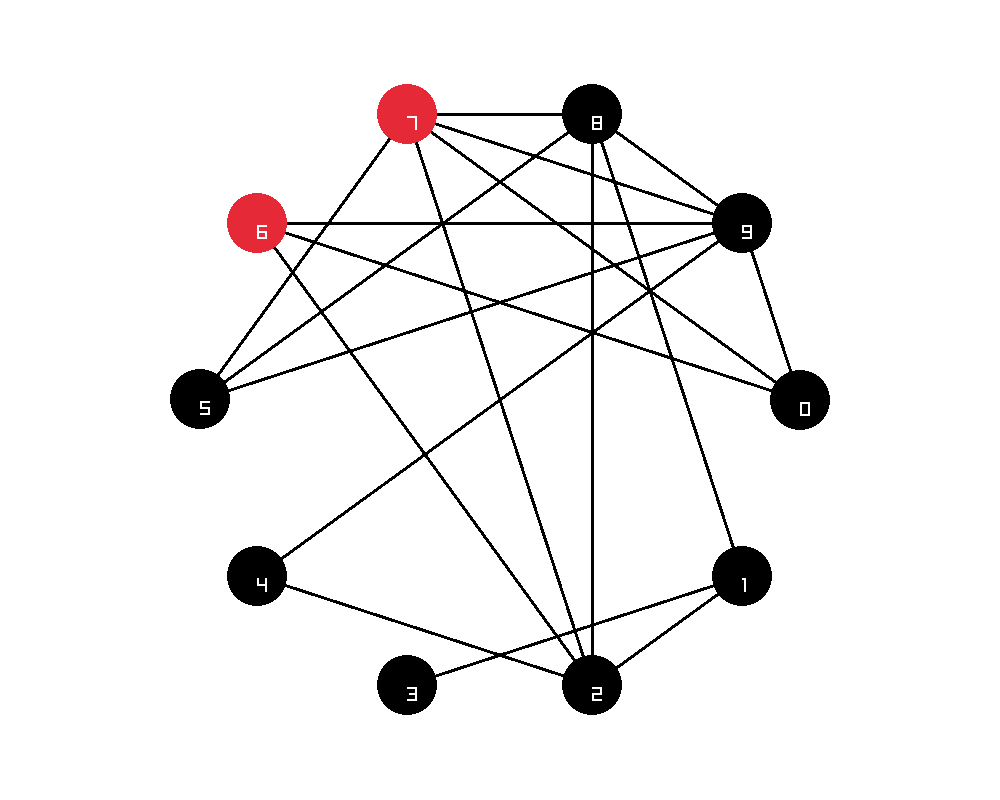
\includegraphics[scale=0.17]{images/colors_it3.png}
    \subcaption{Graf G nakon prve iteracije bojanja}
    \label{prvo_bojanje}
  \end{subfigure}
  \begin{subfigure}[b]{0.4\linewidth}
    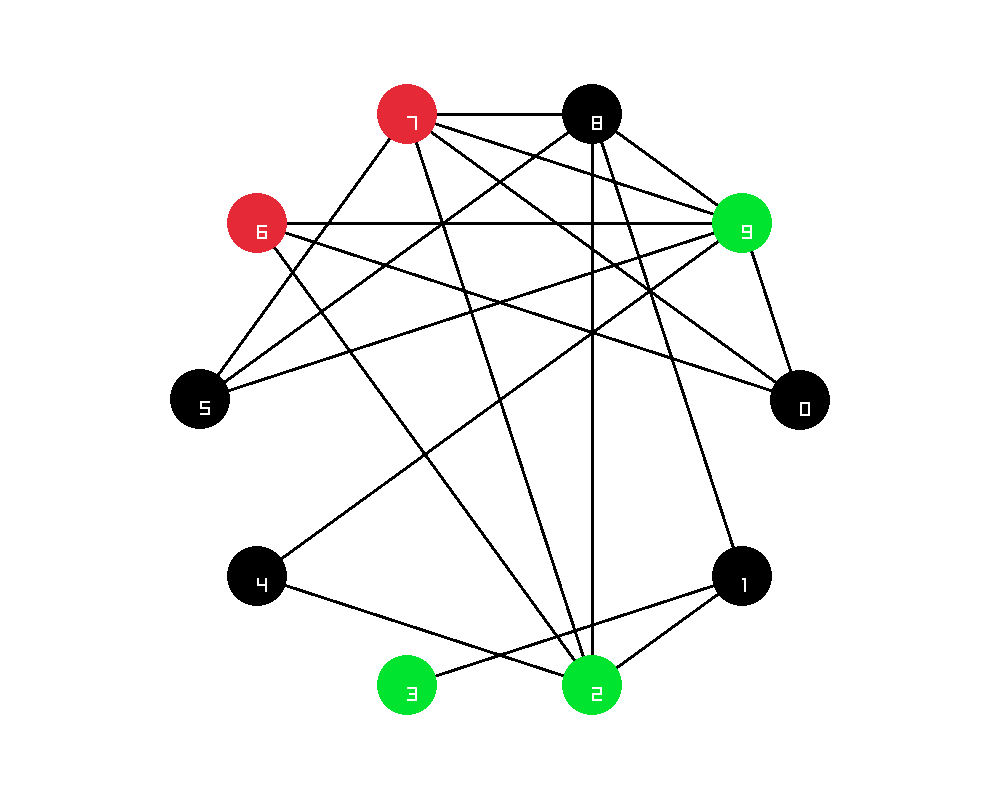
\includegraphics[scale=0.17]{images/colors_it4.png}
    \subcaption{Graf G nakon druge iteracije bojanja}
    \label{drugo_bojanje}
  \end{subfigure}
  \bigskip
  \begin{subfigure}[b]{0.4\linewidth}
    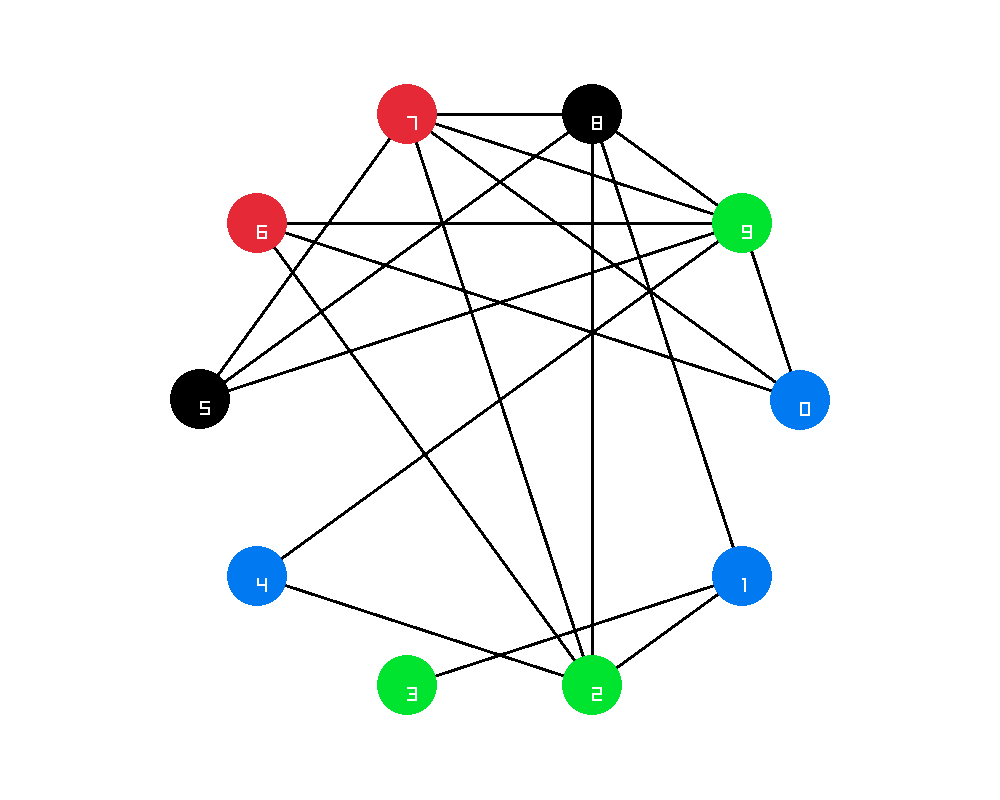
\includegraphics[scale=0.17]{images/colors_it5.png}
    \caption{Graf G nakon trece iteracije bojanja}
    \label{trece_bojanje}
  \end{subfigure}
  \begin{subfigure}[b]{0.4\linewidth}
    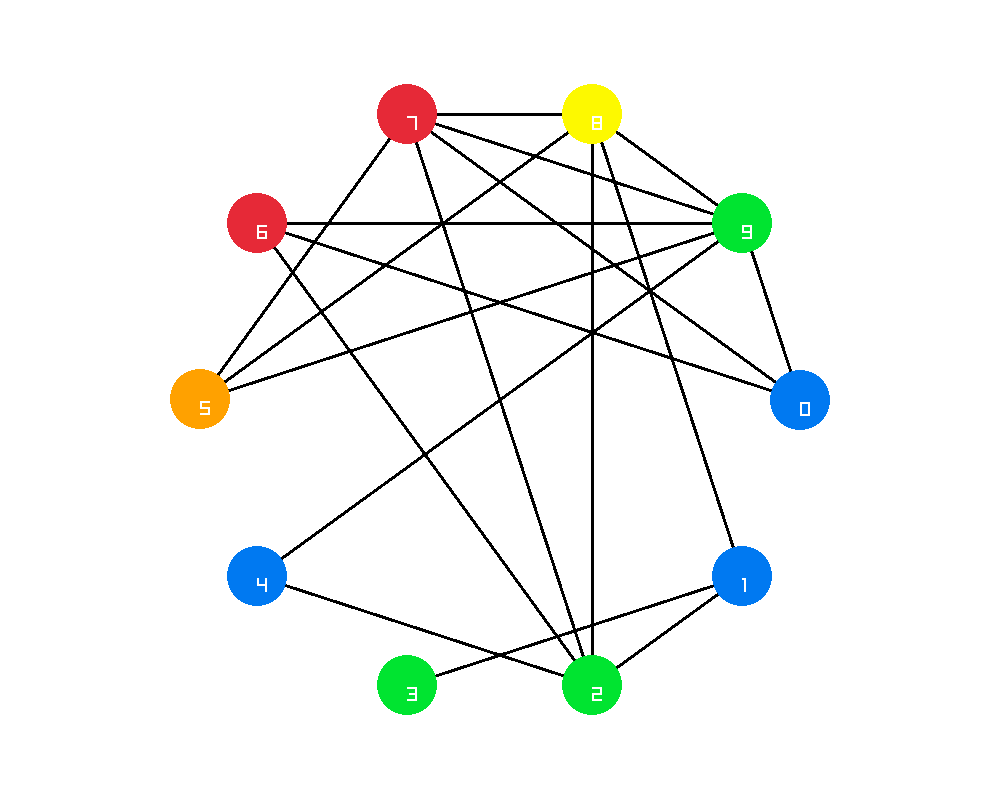
\includegraphics[scale=0.17]{images/colors_it7.png}
    \caption{Konačno bojanje grafa G}
    \label{zadnje_bojanje}
  \end{subfigure}
  \caption{Koraci bojanja grafa G}
\end{figure}

\newpage
\section{Traženje maksimalne klike}
U sklopu rada implementirane su dvije metode traženja maksimalne klike grafa: pohlepno traženje lokalno maksimalne klike kao što je opisano u poglavlju
\ref{pog:greedy_clique} i SDP relaksacijom definiranom u \ref{eq1} pomoću algoritma \ref{maks_clique}. Za graf je određen njegov inverzni graf kojem se
određuje stabilni skup koji je zapravo klika u početnom grafu.

\subsection{Primjer traženja maksimalne klike}
Na slici \ref{fig:klika} prikazana je klika dobivena algoritmom \ref{maks_clique} za graf G prikaz na slici \ref{grafG}. Klika sadrži vrhove 5, 7, 8 i 9.
Ovo klika je ujedno i maksimalna klika grafa G.

U tablici \ref{vekt_clique} prikaza je matrica $V$ koja je dobivena faktorizacijom optimalnog rješenje SDP-a \ref{eq1} za graf G. Prema algoritnu \ref{maks_clique}
generira se slučajan vektor r koju je zapisan u tablici \ref{table_clique_r}. Zatim se računa umnožak matrice $V$ i vektora $r$ te se određuje predznak
svakog elementa vektora umnoška. Ovi predznaci su zapisani u tablici \ref{table_clique_sign}. Za graf G elementi na mjestima 5, 7, 8 i 9 imaju jednaki predznak ($-1$)
kao i dodatan element 10 te oni čine potencijalnu kliku. Provjerom vidimo da svi potrebni bridovi postoje te dobivamo kliku koja je prikazana na slici \ref{fig:klika}.

\begin{figure}
  \centering
  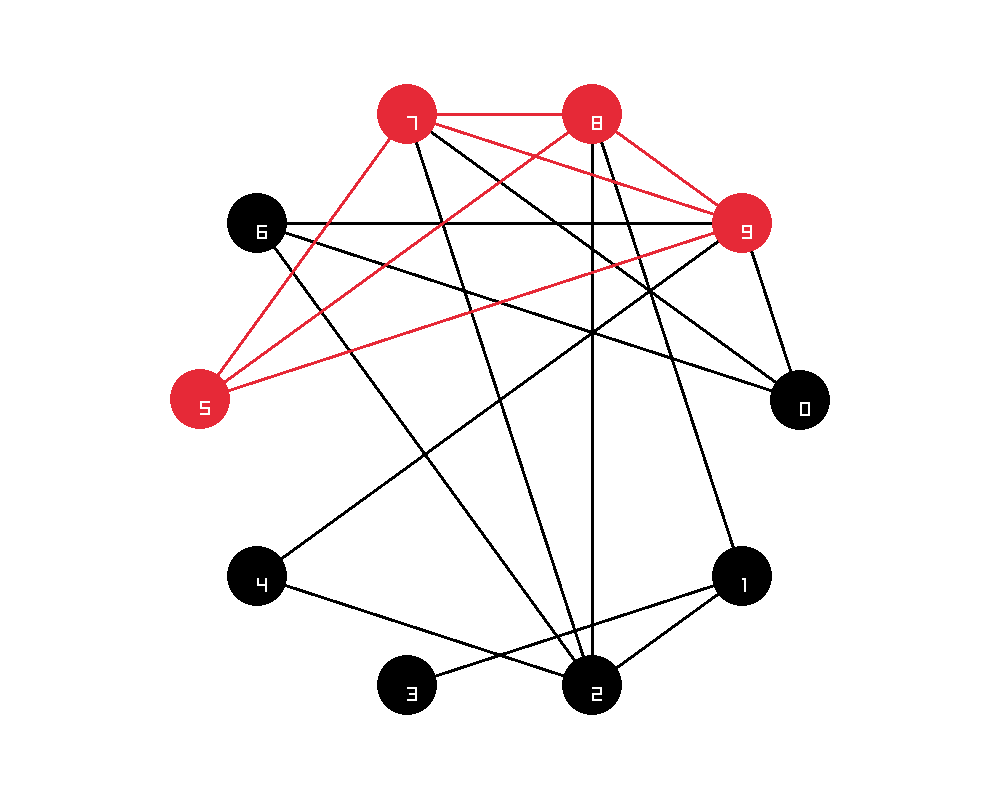
\includegraphics[scale=0.4]{images/max_clique.png}
  \caption{Klika graf G}
  \label{fig:klika}
\end{figure}

\begin{table}[h]
  \caption{Faktorizacija $V$ optimalnog rješenja SDP relaksacije za graf G}
  \label{vekt_clique}
  \centering
  \resizebox{\columnwidth}{!}{
  \begin{tabular}{|c|c|c|c|c|c|c|c|c|c|c|c|}
    \hline
    i & $V_{i,0}$ & $V_{i,1}$ & $V_{i,2}$ & $V_{i,3}$ & $V_{i,4}$ & $V_{i,5}$ & $V_{i,6}$ & $V_{i,7}$ & $V_{i,8}$ & $V_{i,9}$ & $V_{i,10}$ \\
    \hline
    \hline
    0 & 1.000 & 1.000 & 1.000 & 1.000 & 1.000 & -1.000 & 1.000 & -1.000 & -1.000 & -1.000 & -1.000 \\
    \hline
    1 & 1.000 & 1.000 & 1.000 & 1.000 & 1.000 & -1.000 & 1.000 & -1.000 & -1.000 & -1.000 & -1.000 \\
    \hline
    2 & 1.000 & 1.000 & 1.000 & 1.000 & 1.000 & -1.000 & 1.000 & -1.000 & -1.000 & -1.000 & -1.000 \\
    \hline
    3 & 1.000 & 1.000 & 1.000 & 1.000 & 1.000 & -1.000 & 1.000 & -1.000 & -1.000 & -1.000 & -1.000 \\
    \hline
    4 & 1.000 & 1.000 & 1.000 & 1.000 & 1.000 & -1.000 & 1.000 & -1.000 & -1.000 & -1.000 & -1.000 \\
    \hline
    5 & -1.000 & -1.000 & -1.000 & -1.000 & -1.000 & 1.000 & -1.000 & 1.000 & 1.000 & 1.000 & 1.000 \\
    \hline
    6 & 1.000 & 1.000 & 1.000 & 1.000 & 1.000 & -1.000 & 1.000 & -1.000 & -1.000 & -1.000 & -1.000 \\
    \hline
    7 & -1.000 & -1.000 & -1.000 & -1.000 & -1.000 & 1.000 & -1.000 & 1.000 & 1.000 & 1.000 & 1.000 \\
    \hline
    8 & -1.000 & -1.000 & -1.000 & -1.000 & -1.000 & 1.000 & -1.000 & 1.000 & 1.000 & 1.000 & 1.000 \\
    \hline
    9 & -1.000 & -1.000 & -1.000 & -1.000 & -1.000 & 1.000 & -1.000 & 1.000 & 1.000 & 1.000 & 1.000 \\
    \hline
    10 & -1.000 & -1.000 & -1.000 & -1.000 & -1.000 & 1.000 & -1.000 & 1.000 & 1.000 & 1.000 & 1.000 \\
    \hline
  \end{tabular}
  }
\end{table}

\begin{table}
  \caption{Slučajan vektor r}
  \label{table_clique_r}
  \begin{tabular}{|c|c|c|c|c|c|c|c|c|c|c|}
    \hline
    $r_0$ & $r_1$ & $r_2$ & $r_3$ & $r_4$ & $r_5$ & $r_6$ & $r_7$ & $r_8$ & $r_9$ & $r_{10}$\\
    \hline
    \hline
    0.265 & 0.335 & 0.636 & 0.362 & 0.176 & 0.064 & -0.016 & 0.132 & 0.049 & 0.290 & -0.378 \\
    \hline
  \end{tabular}
\end{table}

\begin{table}
  \caption{Predznak umnoška matrice V i vektora r}
  \label{table_clique_sign}
  \begin{tabular}{|c|c|c|c|c|c|c|c|c|c|c|c|}
    \hline
    $r \cdot v_0$ & $r \cdot v_1$ & $r \cdot v_2$ & $r \cdot v_3$ & $r \cdot v_4$ & $r \cdot v_5$ & $r \cdot v_6$ & $r \cdot v_7$ & $r \cdot v_8$ & $r \cdot v_9$ & $r \cdot v_{10}$ \\
    \hline
    \hline
    1 & 1 & 1 & 1 & 1 & -1 & 1 & -1 & -1 & -1 & -1 \\
    \hline
  \end{tabular}
\end{table}

%-------------------------------------------------------------------------------
\chapter{Rezultati i rasprava}
\label{pog:rezultati_i_rasprava}

Za potrebe testiranja napravljen je jednostavan generator slučajnih grafova. Za definirane parametre $n \in \mathbb{N}$ i $p \in [0,1]$, generira
se graf s $n$ vrhova. Bridovi se generiraju slučajno, za svaki brid je vjerojatnost generiranja $p$. Graf je spremljen u datoteku u obliku 
matrice susjedstva. Generiran je po jedan graf za sve $n \in \{5, 10, \dots, 40, 45\}$ i sve $p \in \{0, 0.05, \dots, 0.9, 0.95\}$.

\section{Bojanje grafova}
Svi generirani grafovi obojani su $\delta + 1$ algoritmom i algoritmom zaokruživanja vektorskim projekcijama uz $\epsilon \in \{-0.2, 0, 0.2\}$.
Za algoritam zaokruživanja vektorskim projekcijama, rezultati su izračunati 3 puta te je uzeta najbolja vrijednost. Za svaki algoritam su izračunati prosjeci po
parametru $n$ koji su prikazani u tablici \ref{table:bojanje_n}. Iz tablice vidimo da algoritam zaokruživanja vektorskim projekcijama daje najbolje rezultate za $\epsilon = -0.2$, a
najgore za $\epsilon = 0.2$. Algoritam zaokruživanja vektorskim projekcijama za $\epsilon = -0.2$ i $\delta + 1$ bojanje daju otprilike jednake rezultate. Zanimljivo je primjetiti
da $\delta + 1$ algoritam boja graf s puno manje od $\delta$ boja, pogotovo za veliki $n$.

U tablici \ref{table:bojanje_p}, prikazani su prosječni rezultati po parametru $p$. Vidimo da je SDP relaksacija bolja od $\delta + 1$ bojanja za veliki
$p$ što je za očekivati jer u grafovima generiranima s većim $p$ ima veći broj vrhova koji imaju visoki stupanj.

Dobiveni rezultati za algoritam zaokruživanja vektorskim projekcijama mogli bi se poboljšati korištenjem Wigdersonove tehnike. Implementacijom ove
metode mogli bi se ostvariti bolji rezultati nego korištenjem $\delta + 1$ algoritma.

\begin{table}
  \caption{Broj boja po algoritmu po n}
  \label{table:bojanje_n}
  \centering
  \resizebox{\columnwidth}{!}{%
  \begin{tabular}{|c|c|c|c|c|c|}
    \hline
    n & $\delta +1$ bojanje & SDP bojanje $\epsilon = -0.2$& SDP bojanje $\epsilon = 0$ & SDP bojanje $\epsilon = 0.2$ & $\delta$ \\
    \hline
    \hline
    5 & 2.85 & 2.95 & 3.2 & 3.6 & 3.05\\
    \hline
    10 & 4.25 & 4.5 & 4.7 & 5.8 & 6.45\\
    \hline
    15 & 5.95 & 5.85 & 6.35 & 7.95 & 9.65\\
    \hline
    20 & 7.2 & 7.2 & 7.9 & 10.4 & 12.65\\
    \hline
    25 & 8.1 & 8.3 & 9.65 & 12.4 & 15.5\\
    \hline
    30 & 9.6 & 9.95 & 11.25 & 17.5 & 19\\
    \hline
    35 & 10.6 & 11.25 & 12.65 & 18.65 & 21.5\\
    \hline
    40 & 12 & 12.45 & 13.85 & 21.3 & 24.35\\
    \hline
    45 & 12.65 & 13.55 & 15 & 24.15 & 27    \\
    \hline
  \end{tabular}
  }
\end{table}

\begin{table}
  \caption{Broj boja po algoritmu po p}
  \label{table:bojanje_p}
  \centering
  \resizebox{\columnwidth}{!}{%
  \begin{tabular}{|c|c|c|c|c|c|}
    \hline
    p & $\delta +1$ bojanje & SDP bojanje $\epsilon = -0.2$& SDP bojanje $\epsilon = 0$ & SDP bojanje $\epsilon = 0.2$ & $\delta$ \\
    \hline
    \hline
    0 & 1 & 2.22222 & 4.44444 & 11.7778 & 0 \\
    \hline
    0.05 & 2.55556 & 2.55556 & 4.11111 & 10.6667 & 3.66667 \\
    \hline
    0.1 & 3.44444 & 3.33333 & 4.66667 & 10.4444 & 5 \\
    \hline
    0.15 & 3.88889 & 3.66667 & 5 & 11.3333 & 7.55556 \\
    \hline
    0.2 & 4.66667 & 4.44444 & 5.77778 & 10.3333 & 9.33333 \\
    \hline
    0.25 & 5.44444 & 6 & 6.66667 & 11.3333 & 11.7778 \\
    \hline
    0.3 & 10.8889 & 12 & 13.3333 & 22.6667 & 23.5556 \\
    \hline
    0.35 & 6.44444 & 6.66667 & 7.66667 & 12.3333 & 13.2222 \\
    \hline
    0.4 & 6.66667 & 7.11111 & 8.33333 & 12.1111 & 15.2222 \\
    \hline
    0.45 & 7.22222 & 7.44444 & 8.66667 & 12.6667 & 16.1111 \\
    \hline
    0.5 & 8 & 7.88889 & 9.33333 & 13.2222 & 16.6667 \\
    \hline
    0.55 & 9 & 9 & 10.2222 & 13.4444 & 18.7778 \\
    \hline
    0.6 & 9.66667 & 10.1111 & 10.3333 & 14.3333 & 19.2222 \\
    \hline
    0.65 & 9.66667 & 10.1111 & 10.7778 & 14.6667 & 20.2222 \\
    \hline
    0.7 & 10.3333 & 11 & 11.8889 & 14.7778 & 21.2222 \\
    \hline
    0.75 & 11.2222 & 12.4444 & 12.3333 & 15.6667 & 22.3333 \\
    \hline
    0.8 & 12.3333 & 12.6667 & 13.5556 & 16.3333 & 23.6667 \\
    \hline
    0.85 & 13.4444 & 13.3333 & 14.1111 & 16.5556 & 23.7778 \\
    \hline
    0.9 & 15.1111 & 14.7778 & 15.2222 & 18.3333 & 24.6667 \\
    \hline
    0.95 & 17.1111 & 16.3333 & 16.7778 & 17.8889 & 25 \\
    \hline
  \end{tabular}
  }
\end{table}

\section{Pronalazak maksilne klike}
Za sve generirane grafove određen su klike pohlepnim pronalaskom lokalno maksimalne klike i pronalaskom SDP relaksacijom. Algoritam SDP relaksacije pokrenut je 3 puta
i uzeta je vrijednost maksimalne od pronađenih klika. Prosječne veličine pronađenih klike za svaki $n$ prikazane su u tablici \ref{table:klik_n}
Iz tablice je vidljivo da algoritam baziran na SDP relaksaciji pronalazi veće klike od pohlepnog, otprilike za jedan vrh više po kliki.

U tablici \ref{table:klik_p} prikazane su prosječne veličine pronađenih klika za različite vrijednosti parametra $p$. Za gotovo sve vrijednosti
parametra, SDP relaksacijom se pronalaze veća klika nego pohlepnim algoritmom. Najveća razlika između algoritama je za vrijednosti $p \sim 0.5$.

\begin{table}
  \caption{Veličina pronađene klike po n}
  \label{table:klik_n}
  \centering
  \begin{tabular}{|c|c|c|}
    \hline
    n & pohlepni algoritam & SDP relaksacija \\
    \hline
    \hline
    5 & 2.5 & 2.8 \\
    \hline
    10 & 3.5 & 4.05 \\
    \hline
    15 & 4.45 & 5 \\
    \hline
    20 & 4.7 & 5.6 \\
    \hline
    25 & 5.4 & 6.55 \\
    \hline
    30 & 6 & 7.6 \\
    \hline
    35 & 6.15 & 7.75 \\
    \hline
    40 & 6.85 & 7.65 \\
    \hline
    45 & 6.9 & 7.55 \\
    \hline
  \end{tabular}
\end{table}

\begin{table}
  \caption{Veličina pronađene klike po p}
  \label{table:klik_p}
  \centering
  \begin{tabular}{|c|c|c|}
    \hline
    p & pohlepni algoritam & SDP relaksacija \\
    \hline
    \hline
    0 & 1 & 0.888889 \\
    \hline
    0.05 & 1.77778 & 2.11111 \\
    \hline
    0.1 & 2 & 2.44444 \\
    \hline
    0.15 & 2.33333 & 2.77778 \\
    \hline
    0.2 & 2.33333 & 2.77778 \\
    \hline
    0.25 & 2.66667 & 4 \\
    \hline
    0.3 & 5.33333 & 8 \\
    \hline
    0.35 & 3.44444 & 4.33333 \\
    \hline
    0.4 & 3.44444 & 4.44444 \\
    \hline
    0.45 & 3.77778 & 5.33333 \\
    \hline
    0.5 & 4.22222 & 5.22222 \\
    \hline
    0.55 & 4.77778 & 6.11111 \\
    \hline
    0.6 & 5.66667 & 5.66667 \\
    \hline
    0.65 & 5.55556 & 7 \\
    \hline
    0.7 & 6.11111 & 7.66667 \\
    \hline
    0.75 & 6.55556 & 8.22222 \\
    \hline
    0.8 & 9 & 8.88889 \\
    \hline
    0.85 & 9.44444 & 11.1111 \\
    \hline
    0.9 & 11.6667 & 12.6667 \\
    \hline
    0.95 & 14.7778 & 15.5556 \\
    \hline
  \end{tabular}
\end{table}

\chapter{Upute za prevođenje i pokretanje}
\label{pog:upute_za_prevođenje_i_pokretanje}
\section{Upute za prevođenje}
Prije prevođenja pretpostavlja se da su na računalu instalirani DSDP \cite{dsdp-user-guide}, OpenBLAS \cite{openBLAS} i raylib.
Definiran je \verb|Makefile| pa je moguće prevođenje pomoću naredbe \verb|make|. Ovime nastaju programi \verb|.out/main.out|, \verb|.out/visualize.out|, \verb|.out/generate.out| i 
\verb|.out/tester.out|.

\section{Glavni program}
Program \verb|.out/main.out| glavni je program kojem se putem opcija definira željeni ispis na ekran te putanja do datoteke u kojoj je spremljen
graf. Moguće opcije su ispis bridova grafa, ispis boja grafa obojanog $\delta + 1$ algoritmom, ispis boja grafa obojanog algoritmom zaokruživanja
vektorskim projekcijama, ispis klike pronađene pohlepnim algoritmom i ispis klike pronađene semidefinitnom relaksacijom.

\begin{verbatim}
  usage: main.out [options] file
  options:
  --help         display help
  -print         print graph
  -delta_color   color the graph with delta+1 algorithm
  -color         color the graph with SDP algorithm
  -greedy_clique find clique using greedy algorithm
  -clique        find clique using SDP algorithm
\end{verbatim}

\section{Program za vizualizaciju}
Program \verb|.out/visualize.out| program je za vizualizaciju grafa. Prilikom pokretanja upisuju se opcije vizualizacije i ime datoteke u kojoj je 
spremljen graf. Moguća je vizualizacija obojanog grafa, ili $\delta + 1$ algoritmom ili algoritmom zaokruživanja vektorskim projekcijama. Također je
moguće vizualizirati kliku grafa, pronađenu ili pohlepnim algoritmom ili SDP relaksacijom. Na slici \ref{fig:visualize} prikazani su primjeri
vizualizacije bojanja i maksimalne klike grafova.

\begin{verbatim}
  usage: visualize.out option file
  options:
  --help         display help
  -delta_color   color the graph with delta+1 algorithm
  -color         color the graph with SDP algorithm
  -greedy_clique find clique using greedy algorithm
  -clique        find clique using SDP algorithm
\end{verbatim}


\begin{figure}
  \centering
  \begin{subfigure}[b]{0.4\linewidth}
    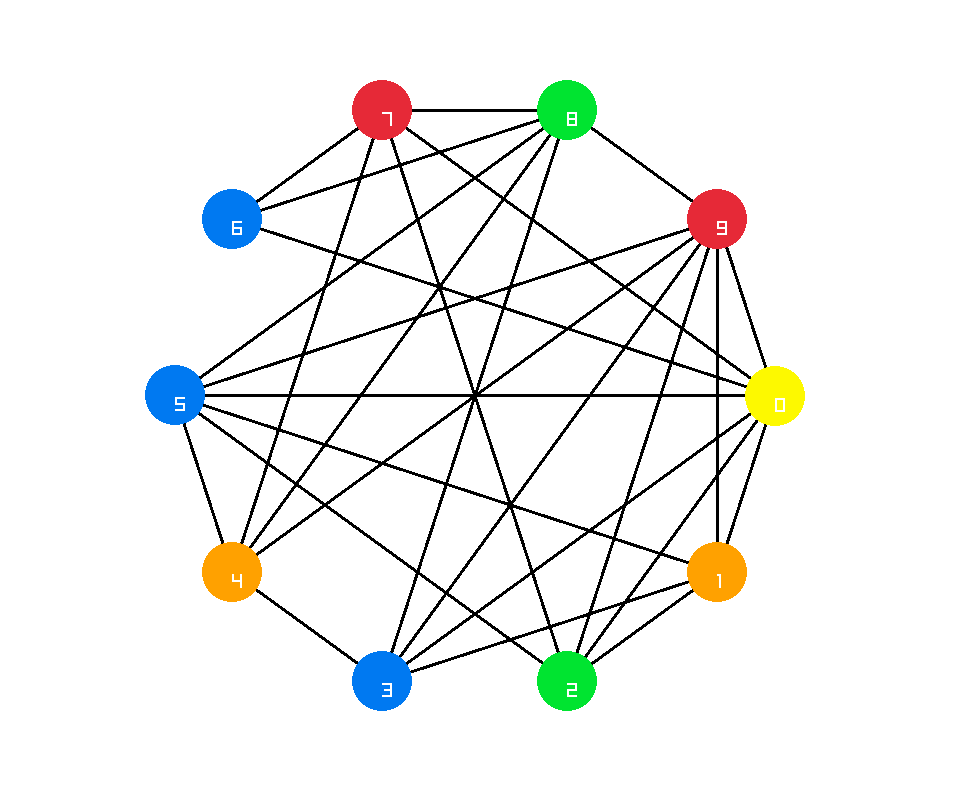
\includegraphics[scale=0.23]{images/color.png}
    \subcaption{Primjer vizualizacije obojanog grafa}
  \end{subfigure}
  \hfill
  \begin{subfigure}[b]{0.4\linewidth}
    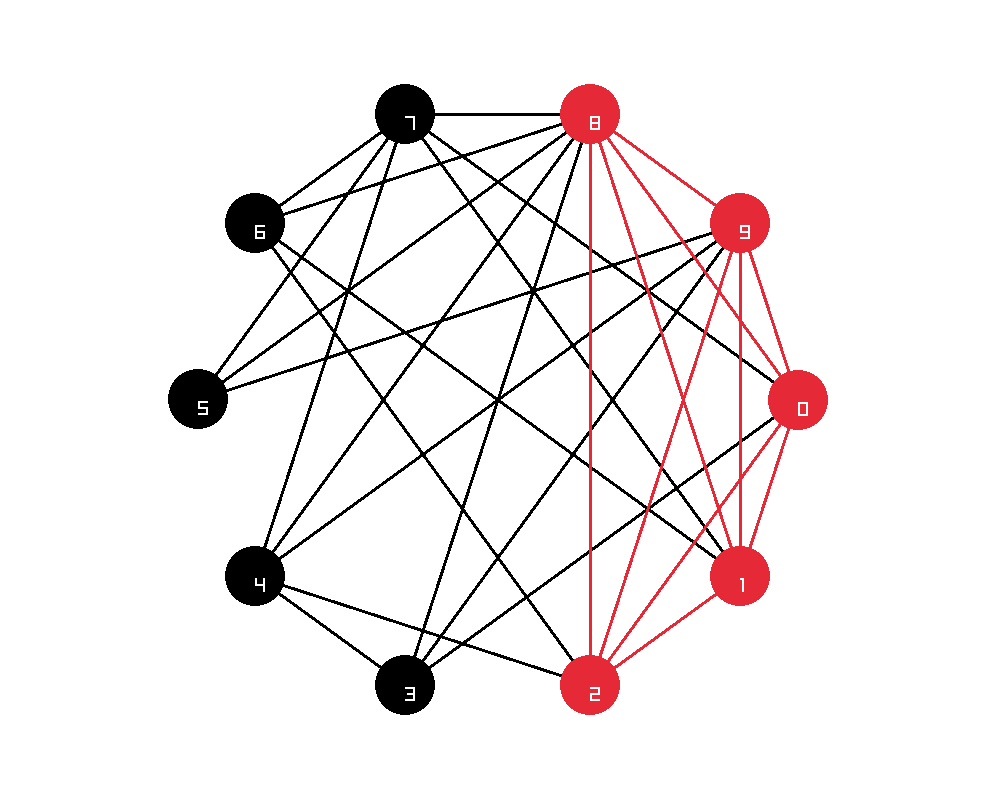
\includegraphics[scale=0.23]{images/clique.png}
    \subcaption{Primjer vizualizacije klike grafa}
  \end{subfigure}
  \caption{Primjeri programa vizualizacije}
  \label{fig:visualize}
\end{figure}


%--- ZAKLJUČAK / CONCLUSION ----------------------------------------------------
\chapter{Zaključak}
\label{pog:zakljucak}
U sklopu rada, dan je pregled problema bojanja grafova i pronalaska maksimalne klike grafa.

Implementirano je bojanje grafova pomoću SDP relaksacije uz algoritam zaokruživanja vektorskim projekcijama i pomoću $\delta + 1$ bojanja. 
Oba algoritma u polinomnom vremenu ispravno bojaju graf, no $\delta +1$ algoritam eksperimentalno daje bolje rezultate.
U danjem radu, bilo bi moguće poboljšati bojanje grafa algoritmom zaokruživanja uz primjenu Wigdersonove tehnike.

Mogle bi se istražiti i implementirati druge formulacije semidefinitnih relaksacija bojanja grafova koje bi se tada usporedile s trenutnim
implementacijama. U danjem radu, trebalo bi implementirati izračun Lovászove theta funkcije kao ocjenu veličine broja boja i maksimalne klike.

Također, implementiran je pronalazak velike klike grafa pomoću semidefinitne relaksacije problema i pomoću
pohlepnog algoritma traženja lokalno maksimalne klike. Algoritam semidefinitne relaksacija pronalazi veće klike.

Ove rezultate trebalo bi usporediti s drugim nekomercijalnim bibliotekama.


%--- LITERATURA / REFERENCES ---------------------------------------------------

% Literatura se automatski generira iz zadane .bib datoteke / References are automatically generated from the supplied .bib file
% Upiši ime BibTeX datoteke bez .bib nastavka / Enter the name of the BibTeX file without .bib extension
\bibliography{literatura}



%--- SAŽETAK / ABSTRACT --------------------------------------------------------

% Sažetak na hrvatskom
\begin{sazetak}
U sklopu rada, dan je opis problema bojanja grafova i pronalaska maksimalne klike grafa. Opisani su jednostavni načini rješavanja
ovih problema. Opisano je formulacija semidefinitnih problema kao i njihova primjena kod bojanja grafova i traženja maksimalne klike.
Objašnjena je važnost Lovászove theta funkcije i dana formulacija semidefinitnog problema za pronalazak njezine vrijednosti.

Implementirano je bojanje grafova pomoću SDP relaksacije uz algoritam zaokruživanja vektorskim projekcijama i pomoću $\delta + 1$ bojanja
i uspoređeni su rezultati. Također, implementiran je pronalazak velike klike grafa pomoću semidefinitne relaksacije problema i pomoću
pohlepnog algoritma traženja lokalno maksimalne klike.

Implementiran je i program za vizualizaciju grafa koji prikazuje obojani graf ili njegovu maksimalnu kliku.

\end{sazetak}

\begin{kljucnerijeci}
  bojanje grafa; semidefinitno programiranje; maksimalna klika; Lovászova fukcija
\end{kljucnerijeci}


% Abstract in English
\begin{abstract}
  In this paper, graph coloring and maximum clique number are described. Simple procedures for
  solving these problems are explained. The formulation of semidefinite problems is given
  and so is their application in graph coloring and finding max clique.
  The importance of Lovász theta function is explained and semidefinite program
  for finding its value is given.

  Graph coloring is implemented using SDP relaxing and rounding via vector projections.
  Graph coloring is also solved using $\delta + 1$ coloring and the results are compared.
  Finding a large clique is also implemented both via semidefinite relaxation
  and using a greedy algorithm of finding locally maximal clique.
  
  Graph visualisation program which shows either a colored graph
  or its maximum clique is implemented.
\end{abstract}

\begin{keywords}
  graph coloring; SDP; maximal clique number; Lovász function
\end{keywords}


%--- PRIVITCI / APPENDIX -------------------------------------------------------

% Sva poglavlja koja slijede će biti označena slovom i riječi privitak / All following chapters will be denoted with an appendix and a letter
\backmatter

\end{document}
